
% ----------------------------------------------------------
% CAPÍTULO 03 - METODOLOGIA E DADOS
% ----------------------------------------------------------

\chapter{Metodologia e dados} \label{cha:metodologia}

Este capítulo descreve os modelos de Equilíbrio Geral Computável e microssimulação comportamental utilizados para estimar os efeitos do comércio internacional sobre a distribuição da renda familiar e os níveis de pobreza no Brasil. Também se apresenta a base de dados usada para a calibragem dos referidos modelos e a implementação da estratégia empírica para simular os efeitos de um choque de liberalização comercial.


\section{O modelo de Equilíbrio Geral Computável} \label{sec:egc}

Utiliza-se o modelo nacional estático de Equilíbrio Geral Computável para o Brasil, o ORANIG-BR, adaptado para cumprir os objetivos propostos nesta dissertação. Esse modelo partiu da estrutura teórica do ORANI \cite{dixit80} e a extensão do PHILGEM \cite{corong12, corong14}. O modelo é da tradição australiana do tipo Johansen, na qual o escopo matemático é concebido a partir de um conjunto de equações linearizadas e as soluções são apresentadas como elasticidades, representando as taxas de crescimento, sendo possível diversos tipos de fechamento.

Sua especificação teórica é composta por blocos de equações que determinam as relações de oferta a partir das hipóteses de otimização e \textit{market clearing}. O modelo incorpora os pressupostos neoclássicos das firmas minimizadoras de custos, famílias maximizadoras de utilidade e equilíbrio dos mercados - esta sendo garantida desde que a oferta e demanda se igualem para o mercado de produtos e serviços domésticos, importados, margens e para o mercado de trabalho.

O uso do modelo de EGC para estudos de análise política, sobretudo sobre impactos e efeitos de algum determinado fenômeno econômico, político ou histórico se tornou cada vez mais frequente na literatura econômica. Há diversos benefícios em trabalhar com esse modelo: é possível operar com altos níveis de desagregação setorial e regional; considerar as relações de interdependência entre os setores e os agentes econômicos; e capturar o efeito-renda e efeito-preço, que estão diretamente relacionados com os canais de transmissão entre comércio internacional e desigualdade de renda e pobreza \cite{anderson20}.

Para esta dissertação, foram realizadas duas principais modificações no modelo ORANIG-BR: 1- o fator trabalho foi dividido em três categorias que refletem os diferentes tipos de força de trabalho a partir do nível de escolaridade; e 2- as famílias são divididas em cem categorias de acordo com a renda. Essa desagregação captura os diferentes impactos que as reformas econômicas têm no mercado de trabalho e na distribuição de renda, assim como as diferentes fontes de renda, respectivamente \cite{carneiro06}.

\subsection{Produção} \label{subsec:producao}

Os setores produtivos seguem os pressupostos neoclássicos de minimização dos custos numa estrutura de mercado de concorrência perfeita, sujeitos a tecnologias de retornos constantes de escala - representadas por funções CES e Leontief. A Figura \ref{fig:estrutura_producao} apresenta a estrutura de produção do modelo. Há cerca de três produtos: 1- bens intermediários; 2- fatores primários; e 3- outros fatores\footnote{"Outros fatores" são as taxas e subsídios do modelo.}. Para se produzir o primeiro, deve-se combinar uma determinada composição das \textit{commodities} disponíveis, decidindo sua origem - se doméstico ou importado. Para produzir o segundo, deve-se combinar quantidades relativas de capital e trabalho, sendo que este é determinado a partir de uma combinação dos três tipos disponíveis de trabalhadores.

Desse modo, para poder produzir nesse modelo, deve-se combinar os bens intermediários, os fatores primários e os outros fatores a partir da minimização dos custos da função Leontief\footnote{Isso implica que esses três fatores são complementares perfeitos, não admitindo substituição}.

\begin{align}
	\underset{i = 1, ... , 124}{Leontief} \{\frac{X_{ij}}{A_{ij}}\} = A_jZ_j, \hspace{2cm} j = 1, ... , 65
\end{align}

No qual $X_{ij}$ corresponde ao insumo $i$ da indústria $j$; $Z_j$ é o nível de atividade da indústria $j$; e $A_ij$ é o coeficiente tecnológico. Se este é igual a 1, significa que é o coeficiente insumo-produto que mostra o insumo mínimo efetivo de $i$ necessário para sustentar uma unidade de atividade na indústria $j$ \cite{dixit80}.

A decisão entre a fonte doméstica ou importada é modelada a partir da hipótese de \textcite{armington69} a qual relaciona os insumos de ambas as fontes como substitutos imperfeitos. Desse modo, para capturar esse efeito, assume-se as unidades de um determinado insumo, diferenciáveis apenas pela fonte, são combinadas para fornecer um só insumo, chamado de \textit{insumo efetivo}:

\begin{align}
	X_{ij} = \underset{s = 1, 2}{CES} = \{\frac{X_{(is)j}}{A_{(is)j}}; \rho_{ij}, b_{(is)j}\}, \hspace{2cm} i & = 1, ... , 124 \\ j & = 1, ... , 65 \notag
\end{align}

No qual $X_{(is)j}$ se refere ao insumo $i$ da fonte $s$ pertencente ao setor $j$; $\rho$ e $b$ são parâmetros de substituição entre as variáveis doméstica e importada. 

\begin{landscape}
	\begin{figure}
		\centering
		
\includegraphics[width=0.8\linewidth]{Imagens/002.ai}
		\caption{estrutura de produção do modelo ORANIG-BR}
		\label{fig:estrutura_producao}
		\footnotesize
		Fonte: elaboração própria (2023)
	\end{figure}
\end{landscape}

\subsubsection{Composição do fator trabalho} \label{}

Como dito anteriormente, o fator trabalho foi subdividido em três grupos: não qualificado, semi-qualificado e qualificado. Esta divisão segue a intuição de que os produtores buscam um determinado conjunto de habilidades no mercado de trabalho que melhor se adeque a demanda do setor produtivo.

Essa habilidade é representada por anos de educação. O Quadro \ref{quad:categoria_trabalho} apresenta a categorização escolhida para desagregar o fator trabalho.

\begin{quadro}[h]
	\centering
	\begin{threeparttable}
		\caption{Categorização do fator trabalho}
		\footnotesize
		\label{quad:categoria_trabalho}
		\begin{tabular}{|| m{3cm} | m{9cm} ||}
			\hline \hline
			\multicolumn{1}{||c|}{\textbf{variável}} & \multicolumn{1}{c||}{\textbf{descrição}} \\ \hline
			não qualificado  & até Ensino Fundamental completo (até quatro anos de estudo) \\ \hline 
			semi-qualificado & até Ensino Médio completo (cinco a doze anos de estudo) \\ \hline
			qualificado      & Ensino Superior (treze anos ou mais de estudo) \\ \hline \hline
		\end{tabular}
		\begin{tablenotes}
			\scriptsize
			\item Fonte: elaboração própria (2023).
		\end{tablenotes}
	\end{threeparttable}
\end{quadro}

\subsection{Demanda das famílias} \label{subsec:demanda_familias}

A demanda é composta por cem famílias representativas, distribuídas por percentis da renda total. Cada família determina uma composição ótima de sua cesta de consumo, escolhendo os insumos de tal maneira a maximizar uma função de utilidade Klein-Rubin sujeita a restrição do orçamento familiar \cite{horridge03}. A Figura \ref{fig:estrutura_familia} apresenta a estrutura da demanda das famílias no modelo ORANIG-BR.

A função Klein-Rubin é não-homotética; ou seja, o aumento da renda altera as participações orçamentárias, mesmo com taxas de preço fixas. O consumo é dividido entre dois bens, "subsistência" e "luxo", de tal maneira que o primeiro detém um consumo fixo e o segundo, residual. Diferentemente da função Leontief, a composição das \textit{commodities} é dado por um LES \cite{horridge03}.

Nesse sistema, participação do gasto acima do nível de subsistência, para cada bem, representa uma proporção constante do gasto total de subsistência de cada família representativa. A função de utilidade é dada por:

\begin{align*}
	U(\bar{X}_1, ... , \bar{X}_{124})
\end{align*}

Sujeito a:

\begin{align}
	&\bar{X}_i = \underset{s = 1, 2}{CES} (\bar{X}_{(is)}), \hspace{2cm} i = 1, ... , 124 \\
	&\sum_{s = 1}^{2} \sum_{i = 1}^{124} \bar{P}_{(is)} \bar{X}_{(is)} = C
\end{align}

\begin{landscape}
	\begin{figure}
		\centering
		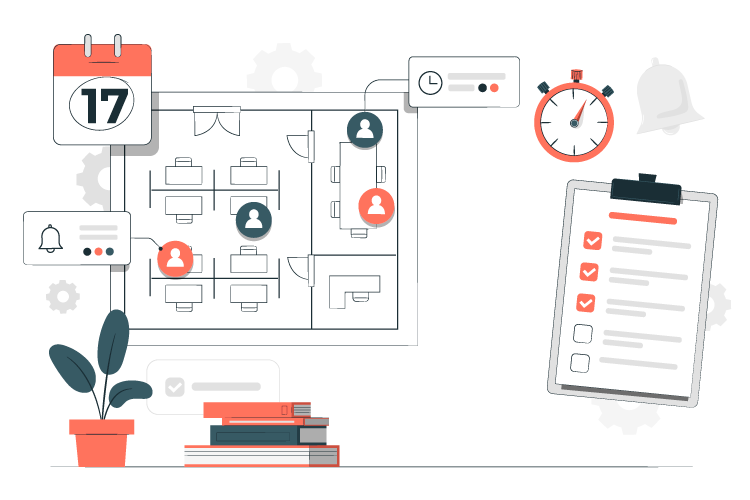
\includegraphics[width=0.8\linewidth]{Imagens/003.ai}
		\caption{estrutura da demanda das famílias do modelo ORANIG-BR}
		\label{fig:estrutura_familia}
		\footnotesize
		Fonte: elaboração própria (2023)
	\end{figure}
\end{landscape}

\subsection{Fechamento do modelo} \label{subsec:fechamento}

Utiliza-se a versão estática do modelo ORANIG-BR porque as vantagens da dinâmica recursiva não seriam aproveitadas neste exercício empírico. O efeito da estrutura produtiva e da distribuição funcional da renda composição que se espera observar pode ser integralmente captado em um modelo estático.

A Figura \ref{fig:fechamento} apresenta o fechamento de curto-prazo adotado no modelo, seguindo as especificações de \textcite{horridge03}. Ou seja, tornou-se exógeno: 1- as variáveis do PIB real - exceto a balança comercial; os fatores produtivos; e 3- as taxas de impostos e distribuição dos investimentos entre as indústrias.

Esse fechamento emula o seguinte comportamento econômico. No curto-prazo, o estoque de capital, a tecnologia e o salário real são exógenos. Isso permite ao modelo determinar o emprego real e, consequentemente, o PIB real. Pelo fato do PIB ser determinado pelo lado da oferta, tendo sua absorção doméstica praticamente formada, a balança comercial, no curto-prazo, ganha a função de ser uma variável de ajuste para a identidade do PIB. Ou seja, o movimento do PIB é determinado pelo movimento da balança comercial.

\begin{landscape}
	\begin{figure}
		\centering
		\includegraphics[width=0.9\linewidth]{Imagens/004.ai}
		\caption{Fechamento de curto-prazo do modelo ORANIG-BR}
		\label{fig:fechamento}
		\footnotesize
		Fonte: elaboração própria (2023)
	\end{figure}
\end{landscape}


\section{Base de dados e calibragem} \label{sec:dados}

A base de dados do modelo foi calibrada a partir da matriz de insumo-produto do sistema de contas nacionais disponível no Instituto Brasileiro de Geografia e Estatística \cite{scn}, contendo 128 produtos e 68 setores econômicos para o ano de 2015. Para esta dissertação, os setores foram agregados em 65 atividades econômicas que produzem 124 produtos. O modelo conta com 114 componentes da demanda final (cem famílias, governo, investimento, exportações e estoque), dois fatores primários (capital e trabalho agregado), três tipos de trabalho (não qualificado, semi-qualificado e qualificado), dois setores de margens (comércio e transporte), e importações por produto para cada um dos 124 produtos.

Foram utilizados os dados da PNAD 2015 \cite{pnad} para desagregar o fator trabalho por anos de educação e os dados da POF 2009 \cite{pof} para detalhar as famílias em cem classes, divididas por percentis da renda total da família. A escolha por essas edições das bases foi motivada pelo fato do modelo ter sido calibrado com esses dados.


\section{Modelo de microssimulação comportamental} \label{sec:microssimulacao}

Como discutido anteriormente, os modelos de equilíbrio geral são utilizados para capturar os efeitos setoriais de variações nos preços relativos e emprego, permitindo focar nos grupos beneficiados e prejudicados a partir de choques exógenos que simulem políticas comerciais, econômicas ou até eventos históricos. Entretanto, sua eficiência é dirimida ao tentar analisar choques distributivos a nível microeconômico \cite{tiberti17}.

Essa limitação está diretamente associada ao pressuposto da Família Representativa dos modelos de equilíbrio geral. Isso implica que o modelo deve assumir uma distribuição relativa de renda intra-grupo constante para todos - o que não é refletido na realidade. A evidência empírica mostra que componente intra-grupo das mudanças observadas na distribuição de renda é, pelo menos, tão importante quanto o componente entre grupos dessas mudanças \cite{colombo08}.

Por essa razão, os modelos de equilíbrio geral, ao não conseguirem captar esses efeitos a nível microeconômico, podem gerar resultados errôneos - sobretudo se tratando de estudos sobre pobreza. Ao não conseguir capturar a heterogeneidade de uma família, o pressuposto da Família Representativa pode acabar por subestimar o efeito dos choques exógenos \cite{colombo08}. 

Uma alternativa é utilizar os modelos de microssimulação integrados ao modelo de equilíbrio geral. Essa combinação é particularmente útil para estudos sobre desigualdade e pobreza em países em desenvolvimento, uma vez que que tanto o foco micro quanto macroeconômico é requerido: o primeiro para ter um cenário detalhado das rendas e despesas a nível individual, além das reações dos indivíduos frente a choques e outras políticas econômicas; o segundo para poder simular os efeitos diretos e indiretos desses choques sobre toda a estrutura econômica \cite{tiberti17, klevmarken22}.

O modelo de microssimulação pode ser entendido enquanto uma grande variedade de técnicas de modelagem por meio das quais o comportamento ou estado dos indivíduos são estimados ou determinados \cite{figari15}. Na literatura econômica, essa integração macro-micro é amplamente utilizada para avaliar os impactos distributivos de choques e políticas macroeconômicos, particularmente
na área de liberalização comercial \cite{carneiro06, ferreira06, raihan10, cicowiez16, mbanda21}.

Desse modo, para estimar os efeitos do comércio internacional sobre a desigualdade de renda e pobreza ao nível microeconômico, deve-se usar os parâmetros obtidos do modelo de equilíbrio geral em uma nova rodada de microssimulações para investigar os prováveis impactos de choques de demanda de exportação, desvalorização cambial, promoção de exportações, choques de produtividade e liberalização comercial sobre o grau de desigualdade de renda no domicílio e nos níveis de pobreza.

A Figura \ref{fig:microssimulacao} apresenta a estrutura da abordagem do modelo integrado.

\begin{landscape}
	\begin{figure}
		\centering
		\includegraphics[width=\linewidth]{Imagens/005.ai}
		\caption{Fechamento de curto-prazo do modelo ORANIG-BR}
		\label{fig:microssimulacao}
		\footnotesize
		Fonte: elaboração própria (2023)
	\end{figure}
\end{landscape}

\subsection{Forma funcional} \label{subsec:forma_funcional}
 
Baseado na abordagem de \textcite{ganuza07}, utiliza-se dois tipos de microssimulação. O primeiro envolve estimar um modelo de equilíbrio parcial de geração de renda familiar por meio de um sistema de equações que determinam a escolha ocupacional, o retorno do trabalho e do capital humano, os preços ao consumidor e outros componentes da renda familiar e individual. A renda total per capita é definida como:

\begin{align}
	ypc_{hi} = \frac{1}{n_h} \left[ \sum_{i = 1}^{n_h} yp_{hi} + yq_h \right] \label{eq:renda}
\end{align}

No qual:

\vspace{0.5cm}

$
\begin{cases}
	n_h     = \text{tamanho da família $h$;} \\
	yp_{hi} = \text{renda do trabalho do indivíduo $i$ da família $h$} \\
	yq_h    = \text{soma de todas os rendimentos familiares não advindos do trabalho}
\end{cases}
$

\vspace{0.5cm}

E o $yq_h$ é definido como:

\begin{align}
	yq_h = \sum_{i = 1}^{n_h} yqp_{hi} + yqt_h 
\end{align}

No qual:

\vspace{0.5cm}

$
\begin{cases}
	yqp_{hi} = \text{rendimento individual não laboral do membro $i$ da família $h$} \\
	yqt_h    = \text{outras rendas familiares}
\end{cases}
$

\vspace{0.5cm}

A segunda equação é baseada no modelo de \textcite{ganuza02}, conhecida na literatura como \textit{occupational choice model}, estimando a probabilidade do indivíduo permanecer ou ingressar no mercado de trabalho após um determinado choque exógeno.

\begin{align}
	\pi = \pi \left( P, U, S, O, W_1, W_2, M \right) \label{eq:mercado_trabalho}
\end{align}

No qual a estrutura do mercado de trabalho é definido em termos de taxas de participação econômica ($P_j$) e desemprego ($U_j$) entre diferentes grupos $j$ da população em idade ativa definida de acordo com sexo e qualificação, a estrutura de emprego (definido por setor de atividade $S$ e categoria profissional $O$) e remuneração $W_1$, bem como nível global de remuneração $W_2$. A composição de habilidades da população é representada pela variável $M$ \cite{ganuza07}.

\subsection{Abordagem empírica} \label{abordagem_empirica}

A estimação da equação \ref{eq:renda} é realizada através do modelo de duas etapas de Heckman \cite{heckman79} para corrigir o viés de seleção implícito numa regressão de salários\footnote{Só tem salário maior que zero aqueles que estão empregados durante o momento da pesquisa.}. Já a estimação da equação \ref{eq:mercado_trabalho} é feita a partir do estimador de máxima verossimilhança, baseado em \textcite{colombo08}.


